% Based on a script by Stefano Rosatti
% author: Lukasz Kidzinski
% email: lukasz.kidzinski@stanford.edu
% Stanford University
% August 2016

% #########################################

\documentclass{beamer}
\usepackage{textpos}
\usepackage{graphicx}
\usepackage{amsmath}
\usepackage{amssymb}
\usepackage{booktabs}

\newcommand{\bT}{\mathbf{T}}
\newcommand{\cP}{\mathcal{P}}
\newcommand{\cS}{\mathcal{S}}
\newcommand{\vsmall}{\vskip 5px}
\newcommand{\vmedium}{\vskip 10px}
\newcommand{\vbig}{\vskip 20px}
\newcommand{\bA}{\mathbf{A}}
\graphicspath{ {img/} }
\usefonttheme{serif}

\usetheme{stanford}
\author[PIN-CHUN, HSU]{ Mingsheng Long$^{12}$, Yue Cao$^1$, Jianmin Wang$^1$, and Michael I. Jordan$^2$ }
\title[Deep Adaptation Networks]{\LARGE Learning Transferable Features with Deep
Adaptation Networks}
\date[May 17, 2017]{International Conference on Machine Learning, 2015}

\begin{document}

\setbeamercolor{itemize item}{fg=red}
\frame{\titlepage}

\begin{frame}[fragile]{Introduction}
\begin{itemize}
\item{Goal: Enhance the transferability of features from task-specific layers}
\item{Proposed a Deep Adaptation Network DAN architecture}
  \begin{itemize}
    \item{General features can generalize well to a novel task; however, for specific features they cannot bridge the domain discrepancy}
  \end{itemize}

\item{Some ways to enhance feature transferability:}
  \begin{itemize}
    \item{By mean-embedding matching, feature transferability can be enhanced substantially}
    \item{Utilizing multi-layer representations across domains in a reproducing kernel Hilbert space}
  \end{itemize}
\end{itemize}
\end{frame}

\begin{frame}[fragile]{Main Breakthrough}
\begin{itemize}
\item{\emph{Generalizes deep CNN to the domain adaptation}}
\item{Deep adaptation of multiple task-specific layers, including output}
\item{Optimal adaptation using multiple kernel two-sample matching}
\end{itemize}
\end{frame}

\begin{frame}[fragile]{Deep Learning For Domain Adaptation}
\begin{itemize}
\item{None or very weak supervision in the \emph{target} task (new domain)}
  \begin{itemize}
  \item{Target classifier cannot be reliably trained due to over-fitting}
  \item{Fine-tuning is impossible as it requires substantial supervision}
  \end{itemize}
\item{Generalize related supervised source task to the target task}
  \begin{itemize}
  \item{Deep networks can learn transferable features for adaptation}
  \end{itemize}
\item{Hard to find big source task for learning deep features from scratch}
  \begin{itemize}
  \item{Transfer from deep networks pre-trained on unrelated big dataset}
  \item{Transferring features from distant tasks better than random features}
  \end{itemize}
\end{itemize}
\begin{figure}[h]
    \centering
    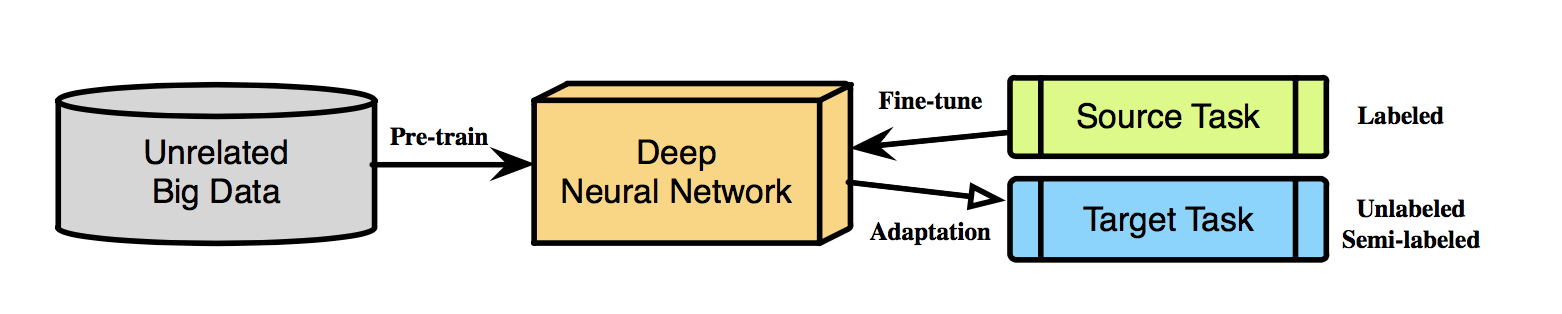
\includegraphics[width=0.95\textwidth]{fig1}
    \caption{\emph{Deep Learning for Domain Adaptation Workflow}}
    \label{fig:mesh2}
\end{figure}
\end{frame}

\begin{frame}[fragile]{How Transferable Are Deep Features?}
\begin{itemize}
  \item{Transferability is restricted by (Yosinski et al. 2014; Glorot et al. 2011)}
  \item{Specialization of higher layer neurons to original task (new task ↓)}
  \item{Disentangling of variations in higher layers enlarges task discrepancy}
  \item{Transferability of features decreases while task discrepancy increases}
\end{itemize}
\begin{figure}[h]
    \centering
    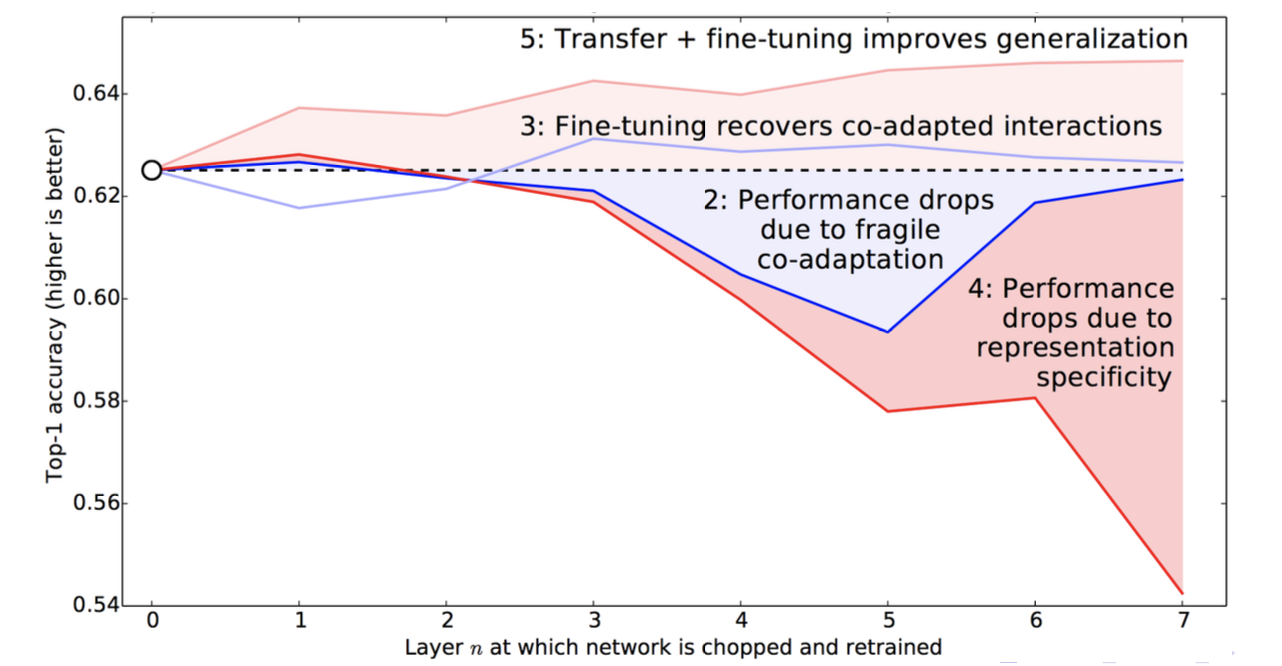
\includegraphics[width=0.4\textwidth]{fig2}
    \caption{Transferability of features decreases while task discrepancy increases}
    \label{fig:mesh2}
\end{figure}
\end{frame}

\begin{frame}[fragile]{Deep Adaptation Network (DAN)}
\begin{block}{Key Observations (AlexNet) (Krizhevsky et al. 2012)}
\begin{itemize}
  \item{Comprised of five convolutional layers $conv1-conv5$ and three fully connected layers $fc6-fc8$}
  \item{Convolutional layers learn general features: safely transferable} 
  \begin{itemize}
  \item{Safely freeze $conv1-conv3$ \& fine tuned $conv4-conv5$}
  \end{itemize}
  \item{Fully-connected layers fit task specificicy: \emph{NOT} safely transferable} 
  \begin{itemize}
  \item{Deeply adapt $fc6-fc8$ using statistically optimal two-sample matching}
  \end{itemize}
\end{itemize}
\end{block}
\begin{figure}[h]
    \centering
    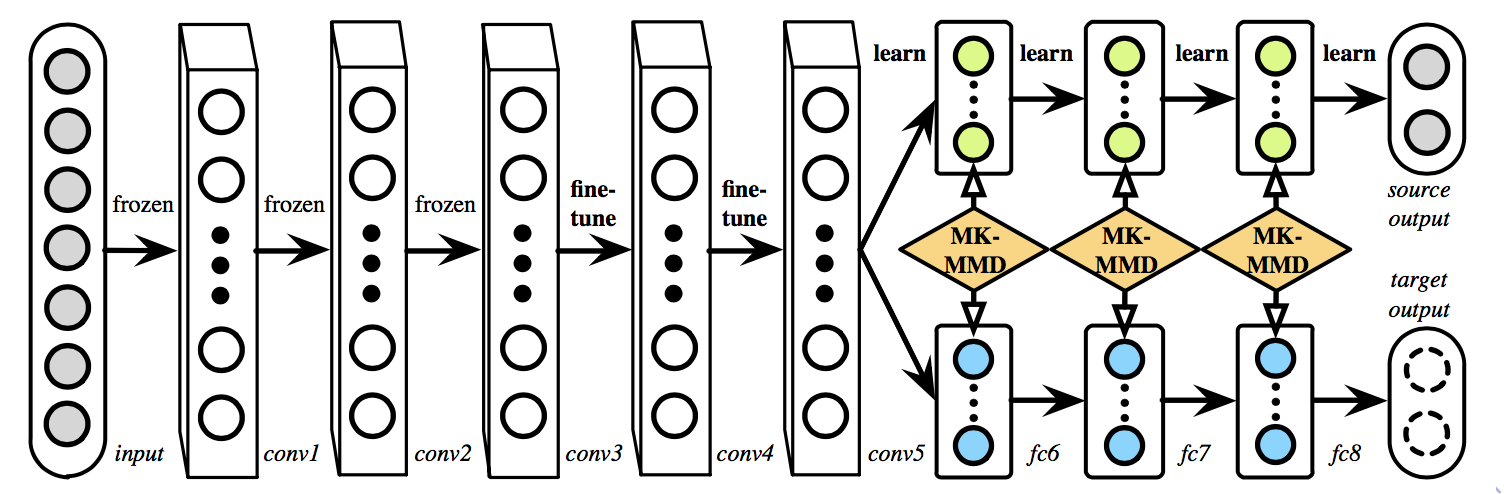
\includegraphics[width=0.4\textwidth]{fig3}
    \caption{The DAN architecture for learning transferable features }
    \label{fig:mesh2}
\end{figure}
\end{frame}

\begin{frame}[fragile]{Objective Function}

\begin{block}{Main Problems}
\begin{itemize}
\item{Feature transferability decreases with increasing task discrepancy}
\item{Higher layers are tailored to specific tasks, NOT safely transferable}
\item{Adaptation effect may vanish in back-propagation of deep networks}
\end{itemize}
\end{block}

\begin{block}{Deep Adaptation with Optimal Matching}
\begin{itemize}
\item{Deep adaptation: match distributions in multiple layers includingoutput}
\item{Optimal matching: maximize two-sample test of multiple kernels}
\end{itemize}
\begin{equation}
\min\limits_\Theta\max\limits_\kappa\frac{1}{n_a}\sum\limits_{i=1}^{n_a}J(\theta(x_i^a),y_i^a)+\lambda\sum\limits_{\ell=l_1}^{l_2}d_k^2(D_s^\ell,D_t^\ell)
\end{equation}
$\lambda > 0$ is a penality, $D_*^\ell=\{h_i^{*\ell}\}$ is the $\ell$-th layer hidden representaion
\end{block}

\end{frame}
\begin{frame}[fragile]{MK-MMD}
\begin{block}{Theorem (Two-Sample Test (Gretton et al. 2012))}
\begin{itemize}
\item{$p=q$ iff $d^2_k(p,q)=0$ (In practice,  $d^2_k(p,q)<\epsilon$})
\item{$\max\limits_{k \in \kappa}d_k^2(D_s^\ell,D_t^\ell)\sigma_k^{-2} \Leftrightarrow$ minType II Error ($d^2_k(p,q)<\epsilon$ when $p\neq q$)}
\end{itemize}
\end{block}
\begin{block}{Multiple Kernel Maximum Mean Discrepancy (MK-MMD)}
$\triangleq$ RKHS distance between kernel embeddings of distributions p and q
\begin{equation}
d_k^2(p,q)\triangleq \lVert E_p[\phi(x^s)]-E_q[\phi(x^t)] \rVert_\mathcal{H_\mathrm{k}}^2
\end{equation}
$k(\mathbf{x}^s,\mathbf{x}^t)=\langle\phi(\mathbf{x}^s), \phi(\mathbf{x}^t)\rangle$ is a convex combination of m PSD kernels
\begin{equation}
\kappa\triangleq\Bigg\{k=\sum\limits_{u=1}^m\beta_uk_u:\sum\limits_{u=1}^m\beta_u=1,\beta_u\geq0,\forall u\Bigg\}
\end{equation}
\end{block}

\end{frame}
\begin{frame}[fragile]{Learning CNN}
\begin{block}{Linear-Time Algorithm of MK-MMD (Streaming Algorithm)}
$O(n^2):d_k^2(p,q)=\mathbf{E}_{\mathbf{x}^s\mathbf{x}\prime^s}k(\mathbf{x}^s,\mathbf{x}\prime^s)+\mathbf{E}_{\mathbf{x}^t\mathbf{x}\prime^t}k(\mathbf{x}^t,\mathbf{x}\prime^t)-2\mathbf{E}_{\mathbf{x}^s\mathbf{x}^t}k(\mathbf{x}^s,\mathbf{x}^t)$
$d_k^2(p,q)=\frac{2}{n_s}\sum\nolimits_{i=1}^{\frac{n_s}{2}}g_k(\mathbf{z}_i) \to$ linear-time unbiased estimate
\begin{itemize}
\item{Quad-tuple: $\textbf{z}_i\triangleq (\textbf{x}_{2i-1}^s, \textbf{x}_{2i}^s, \textbf{x}_{2i-1}^t, \textbf{x}_{2i}^t)$}
\item{$g_k(\textbf{z}_i) \triangleq k(\textbf{x}_{2i-1}^s, \textbf{x}_{2i}^s) + k(\textbf{x}_{2i-1}^t, \textbf{x}_{2i}^t) - k(\textbf{x}_{2i-1}^s, \textbf{x}_{2i}^t) - k(\textbf{x}_{2i}^s, \textbf{x}_{2i-1}^t)$}
\end{itemize}
\end{block}
\begin{block}{Stochastic Gradient Descent(SGD)}
For each layer $\ell$ and for each quad-tuple $\textbf{z}_i\triangleq (\textbf{x}_{2i-1}^s, \textbf{x}_{2i}^s, \textbf{x}_{2i-1}^t, \textbf{x}_{2i}^t)$
\begin{equation}
\nabla_{\Theta^\ell}=\frac{\partial{J(z_i)}}{\partial\Theta^\ell}+\lambda\frac{\partial g_k(z_i^\ell)}{\partial \Theta^\ell}
\end{equation}
\end{block}

\end{frame}
\end{document}
